\section{Evaluation}
\label{sec:evaluation}

\subsection{Experimental Setup}

We perform a quantitative evaluation to evaluate
the scalability of our techniques as well as the quality
of the text, comparisons, and the summaries generated.
For the Text Generation and Trace Comparison evaluation,
all results were collected on
an Intel i7-core 3.1GHz processor machine with 32GB of RAM.
For the Trace Summarization evaluation, all results were
collected on an Intel(R) Xeon (R) CPU E5-2690 v3 @ 2.60GHz
with 56GB RAM and an NVIDIA GK210GL [Tesla K80] GPU.

In addition to the quantitative evaluation, we also
performed a qualitative evaluation by conducting
an informal user study with 1 user who is one of the 
leading experts in distributed tracing. Due to time restrictions,
the user was only able to provide feedback about the text generation
and trace comparison techniques.

\subsection{Text Generation}

\begin{figure}[tbh]
    \centering
    \includegraphics[width=\linewidth]{"fig/summary_cdf"}
    \caption{CDF of generating text for all the traces in the DeathStarBench dataset}
    \label{fig:summary_cdf}
\end{figure}

\fakepara{Quantiative Analysis} To measure the efficiency of our text generation approach, we measure the time taken
to generate the text for every trace in the DeathStarBench dataset. \autoref{fig:summary_cdf}
shows the CDF of the breakdown of the total time taken to generate the text. The time taken
to generate the text is dominated by the time taken to load the data from the backend server.
However, once the data is available, the time taken to generate the text is less than 10 milliseconds
for all traces.

\fakepara{Qualitative Analysis} To evaluate the quality of the text generated, the user mentioned the following:\textcolor{red}{``The first sentence is the interesting one here; the rest of the sentences are a bit difficult to parse.
The interesting parts of the first sentence are the comparisons to general statistics about the trace dataset.  I like the last sentence, because it's starting to push towards deriving a 
root cause for the latency (ie, contention with other tasks), and I think when it's presented as text that's a very digestable representation (vs. some sort of visual interface)."}
This suggests that the expert user believes that the overview paragraph is very useful for explaining root causes of potential problems and does so better than a potential
visual interface might. Although, we can still improve our overview by performing comparison for more statistics that a user might care about. Additionally,
the expert user also suggested \textcolor{red}{``to prune away any boring information and try to get at any root causes (or simply say that the request was normal)"}. This suggests
that text that the execution information being shown to the user is too verbose and we might need to infer some high-level information about the trace instead.

\subsection{Trace Summarization}

\begin{figure}
    \centering
    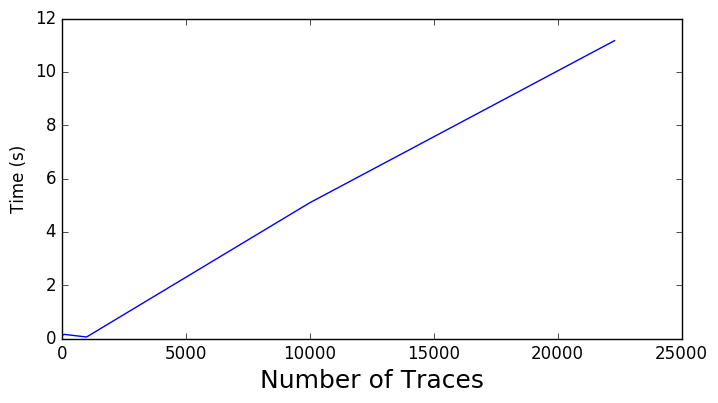
\includegraphics[width=\linewidth]{fig/preprocessing}
    \caption{Time taken for preprocessing traces for summarization}
    \label{fig:preprocessing}
\end{figure}

We explored three metrics to evaluate the summarization of traces. 
First to determine how reasonable our summarization method is we performed a scalability microbenchmark using a single task from multiple traces. 
Then we measure the quality of the summary based on the number of unique sentences it was able to capture from the original documents.
Finally, we perform a macro-scalability test by summarizing all tasks from multiple traces. For each metric we run our own algorithm as well as the potara\footnote{Tool available at \url{https://github.com/sildar/potara} } summarization tool
as a baseline. We chose this tool as this was the only open-source multi-document summarizer that we could find that would run out of the box on our data.
We also tried using BERT but could not properly configure it to generate meaningful summaries.
In addition we also measured how long does it take to perform the preprocessing step. \autoref{fig:preprocessing} shows that the preprocessing
time grows linearly with the number of traces.

\begin{table}[]
    \begin{tabular}{|l|l|l|}
    \hline
    \makecell{\# of Docs} & \makecell{OS} & \makecell{Potara}    \\
    \hline
    \hline
    5                   & 0.103          & 77.429    \\
    \hline
    10                  & 0.105          & 160.240   \\
    \hline
    25                  & 0.107          & 404.716   \\
    \hline
    100                 & 0.109          & 1711.283  \\
    \hline
    500                 & 0.140          & 18118.918 \\
    \hline
    \end{tabular}
    \caption{Time (in s) taken by Potara and Our Summarizer (OS) to summarize varying number of documents for a task}
    \label{tab:micro}
\end{table}

\fakepara{Micro-scalability} We tested the scalability of the summarizers at a document-level. We split up the summarization to be at a task level. 
This means that each task in a given summarization job will have its own set of documents. 
To perform a micro-scalability evaluation we looked at only a single task's documents. For this benchmark, we chose a task that appeared in a large number of traces
so that we can get a better estimate about the scalability of summarizing a large number of documents for a task. 
We ran the summarization algorithm on an increasing number of documents for a particular task. \autoref{tab:micro} shows that potara is unusable after
about 100 traces, and that our summarizer increases sublinearly with the number of documents for a particular task.

\begin{table}[]
    \begin{tabular}{|l|l|l|}
    \hline
    Num Traces & OS    & Potara    \\ \hline \hline
    5          & 0.109 & 31.401    \\ \hline
    10         & 0.116 & 43.979    \\ \hline
    25         & 0.120 & 625.489   \\ \hline
    100        & 0.156 & 6096.836  \\ \hline
    1000       & 0.483 & 72176.924 \\ \hline
    10000      & 3.851 & DNF       \\ \hline
    22290      & 8.224 & DNF       \\ \hline
    \end{tabular}
    \caption{Time taken (in s) by Our Summarizer (OS) and Potara to summarize a varying number of traces}
    \label{tab:macro}
\end{table}

\fakepara{Macro-scalability} While it is important to know how a summarizer works at a document level, we are summarizing entire sets of traces. Therefore
we ran scalability experiments where an increasing number of traces were summarized. Since traces can have multiple tasks, this means that each summarization job 
in this experiment is actually running multiple times, once for each task, before it is considered complete. We ran these experiments on sets with varying number of traces.
\autoref{tab:macro} shows the results for the benchmark. Similar to the micro-scalability benchmarks, it is important to note the lack of scalability in potara. 

\begin{table*}[]
    \begin{tabular}{|l|l|l|l|l|}
    \hline
    Number of documents & Num Matched Sentences - Potara & Num Matched Sentences - OS & Total Sentences \\
    \hline
    \hline
    5                   & 4                              & 16                         & 16              \\
    \hline
    10                  & 5                              & 19                         & 19              \\
    \hline
    25                  & 7                              & 19                         & 19              \\
    \hline
    100                 & 7                              & 20                         & 20              \\
    \hline
    500                 & 8                              & 20                         & 20              \\
    \hline
    \end{tabular}
    \caption{Quality comparison of the summary generated by Potara and Our Summarizer (OS) for varying number of documents for a given task}
    \label{tab:quality}
\end{table*}

\fakepara{Summary Quality} We determined our summaries should be able to capture a general idea of the ``regular'' execution state of the task being summarized. 
A task may have hundreds of sentences in its documents, but only 20 that are unique. As a metric for summary quality
we checked how many of the unique sentences in a task's corpus were present in a summary. \autoref{tab:quality} shows that Potara is not able to capture 
the general idea of a regular execution because at max it is using less than 50\% of the unique sentences in a tasks corpus of sentences.

\subsection{Trace Comparison}

\begin{table}[]
    \begin{tabular}{|c|c|}
    \hline
    Trace Pair                              & Distance \\
    \hline
    \hline
    Identical Traces                        & 0.0      \\
    \hline
    \makecell{Non-Error traces of \\ same type (API)}     & 258.0    \\
    \hline
    \makecell{1 Error, 1 Non-Error \\ trace of same type (API)} & 1610.0  \\
    \hline
    Traces of different type (API)          & 1815.0   \\
    \hline
    \end{tabular}
    \caption{Measured Distance based on our distance function for randomly chosen pairs of traces.}
    \label{tab:comparison_dist}
\end{table}

\fakepara{Quantiative Analysis} We first measured the amount of time taken to generate the diff between the text representations
of two traces. From the DeathStarBench, we randomly chose 100 different pairs of traces and measured the time taken
to generate the diff between the trace. On average, it took 4.87 milliseconds to generate the diff and measure the distance
between two pairs of traces.

\fakepara{Accuracy of Distance function} We wanted to ensure that the distance function we had come up behaves in the expected way
when computing the distance between pairs of traces. \autoref{tab:comparison_dist} shows our detailed results. First,
the distance function returns 0 when computing the distance between two identical traces. Furthermore, the distance function
grows monotonically with increase in deviation between traces. 

\fakepara{Qualitative Analysis of Diff} Regarding the quality of the comparison generated, the user mentioned the following:\textcolor{red}{``This is really cool, I'm actually 
surprised how amenable the complex trace data is to being represented as text.  I've always wondered how to visually compare two traces;I 
really like how you've leveraged some of the more established visual indicators of text comparison (the green+ / red- idiom). With trace diff,
I understand now why having a more verbose trace representation in text is useful.  It's not interesting by itself, but the diffs provide 
context for honing in on specific parts of the text.''} This suggests that the trace diff that we generated using text diff is successful.
However, we do believe that it has certain limitations that we discuss in \autoref{sec:discussion}.
